% Subsystem report for Power Supply system, typeset for the LaTeX processor.
\fancyfoot[R]{MM}
\section [Power]{Power Subsystem}
\subsection{Description}

The power system \index{power} provides reliable, standalone power to all other hardware subsystems. The design supports three different voltage levels as the ATMEGA8518 MCU, analog signal conditioner, and WT32 Bluetooth \textregistered module all require different reference voltages. The source has the flexibility to operate from battery or, when interfaced with a standard USB port, charge the in-system battery and provide uninterrupted power when switching between the two.  

\subsection{System Power Requirements}

Each subsystem requires a different supply voltage as shown in Table \ref{tab:power requirements}. 
\begin{table}[bhp]
\caption[Power Requirements]{Recommended DC operating voltages for ATMEGA8515\cite{ds:ATMEGA8515} and WT32\cite{ds:WT32}}
\small
\begin{center}
\begin{tabular}{l| c c}
\setlength{\tabcolsep}{1pt}
	Device     & Minimum   & Maximum \\\hline
	ATMEGA8515 & 2.7 V     & 5.5 V   \\             
	Analog Signal 
	Conditioner& -12 V     & +12 V\\            
  \small{ADC}& N/A		   & Quiet 3 V\\
	WT-32      & 2.5 V     & 4.4 V            
\end{tabular}
\end{center}
\label{tab:power requirements}
\end{table}

\subsection{Battery}

Taken into consideration are three potential in-system, rechargeable battery\index{battery} supply options: Alkaline, NiMH, or Li-Poly. For some of the basic metrics taken into consideration see table \ref{tab:battery comparison}. Alkaline batteries in series are not a bad option as it would provide the 3V DC source necessary for the MCU/SCU and a similar arrangement could provide power for the other sub-systems as well. The issue with this approach is efficient in-system charging. As with all of the rechargeable batteries considered, use of multiple-cells in a charging system require some intelligent monitoring of each cell to assure that no cell is too far out of sink which can result in overcharging or reverse-charging as a charged cells will rapidly discharge into the uncharged cell. Overcharging can, at the least, damage the battery if not resulting in a dangerous explosion due to an un-containable build up of gaseous bi-products. Another drawback to Alkaline is that voltage output degrades linearly over time which is unfavorable for high-drain electronics. 

NiMH batteries maintain a more consistent voltage over time but have a relatively low efficiency. The best battery solution for this design is the Li-Poly as it not only has a superior efficiency, a single cell outputs a nominal voltage of 3.7 V DC which is acceptable for directly powering the WT-32 Bluetooth \textregistered module. As an added bonus, the WT-32 has a built-in battery charging application as it is often utilized with integrated single cell Li-Poly batteries (i.e. - Bluetooth \textregistered headsets, cell phones). 
  
\begin{table}[bhp]
\caption[Common Battery Types]{Comparison of Common Battery Types\cite{web:bat-tech}}
\small
\begin{center}
\begin{tabular}{l| c c c}
\setlength{\tabcolsep}{1pt}
	Battery     & Single Cell Voltage   & Efficiency & No. of Cycles\\\hline
	Alkaline & 1.5 V                    & 99.9\%        & 100 - 1000\\             
	NiMH     & 1.2 V                    & 66.0\%        & 1000      \\            
  Li-Poly  & 3.7 V		                & 99.8\%        & 500 - 1000 
\end{tabular}
\end{center}
\label{tab:battery comparison}
\end{table}

\subsection{DC/DC Converter}

The Li-Poly battery integrated with the WT32 Bluetooth \textregistered module provides a level 3.7 V DC source which must be re-leveled and distributed to the other sub-systems with as little ripple as possible. Component selection for this application takes into consideration the need for high efficiency. DC-DC converter packages are cheap and readily available so the alternative of building a custom supply is unnecessary. Low-power DC DC converters come in two basic varieties: fixed and adjustable. The adjustable converters feature a built-in gain setting resistor for the internal op-amp and in the case of the LT1073, only three passives are required to configure the device. Refer to figure \ref{fig:general step-up} for an example of the fixed output implementation.

\begin{figure}[hbp]
\centering
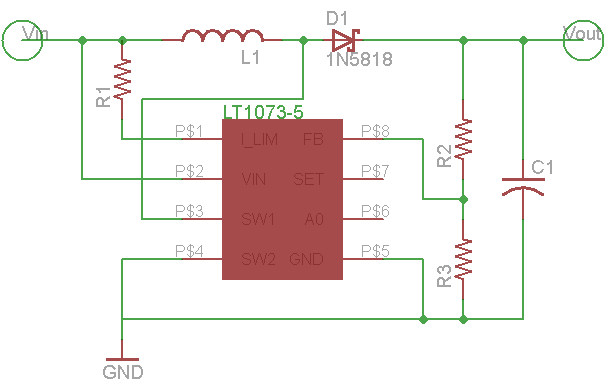
\includegraphics[width=4in]{../drawings/power_gen_fixed.png}
\caption[LT1073 Fixed Output Configuration]{LT1073 general fixed output configuration\cite{ds:lt1073}}
\label{fig:general step-up}
\end{figure}

The datasheet for the LT1073 includes straightforward equations for deciding what values are necessary for the passive components depending on the desired output voltage and current. The standard configurations for the fixed voltage step-up converters from 3V to 5V and 12V are sufficient if the components are up to specification. Namely, the inductor must be able to buffer the input voltage when switching on or off. The inductor must have a low resistance to avoid wasting energy and must not saturate. 

\subsection{Prototyping}

Prototyping the power subsystem is most effectively accomplished using protoboard and a wire wrapping tool. Using DIP wire wrap sockets for the passives required for the LT1073 DC-DC converter allows for fast tweaking if output voltages are not within expected tolerances. The working prototype currently supports the WT32 and ATMEGA8518 power requirements. This prototype may also be powered either via the integrated Li-Poly battery cell or standard USB connection. The Li-Poly battery leverages the WT32 built-in charging system. Future expansions will include the +/- 12V DC power support for the Analog Input Module as shown in Figure \ref{fig:final_power_schematic} .

\begin{figure}[hbp]
\centering
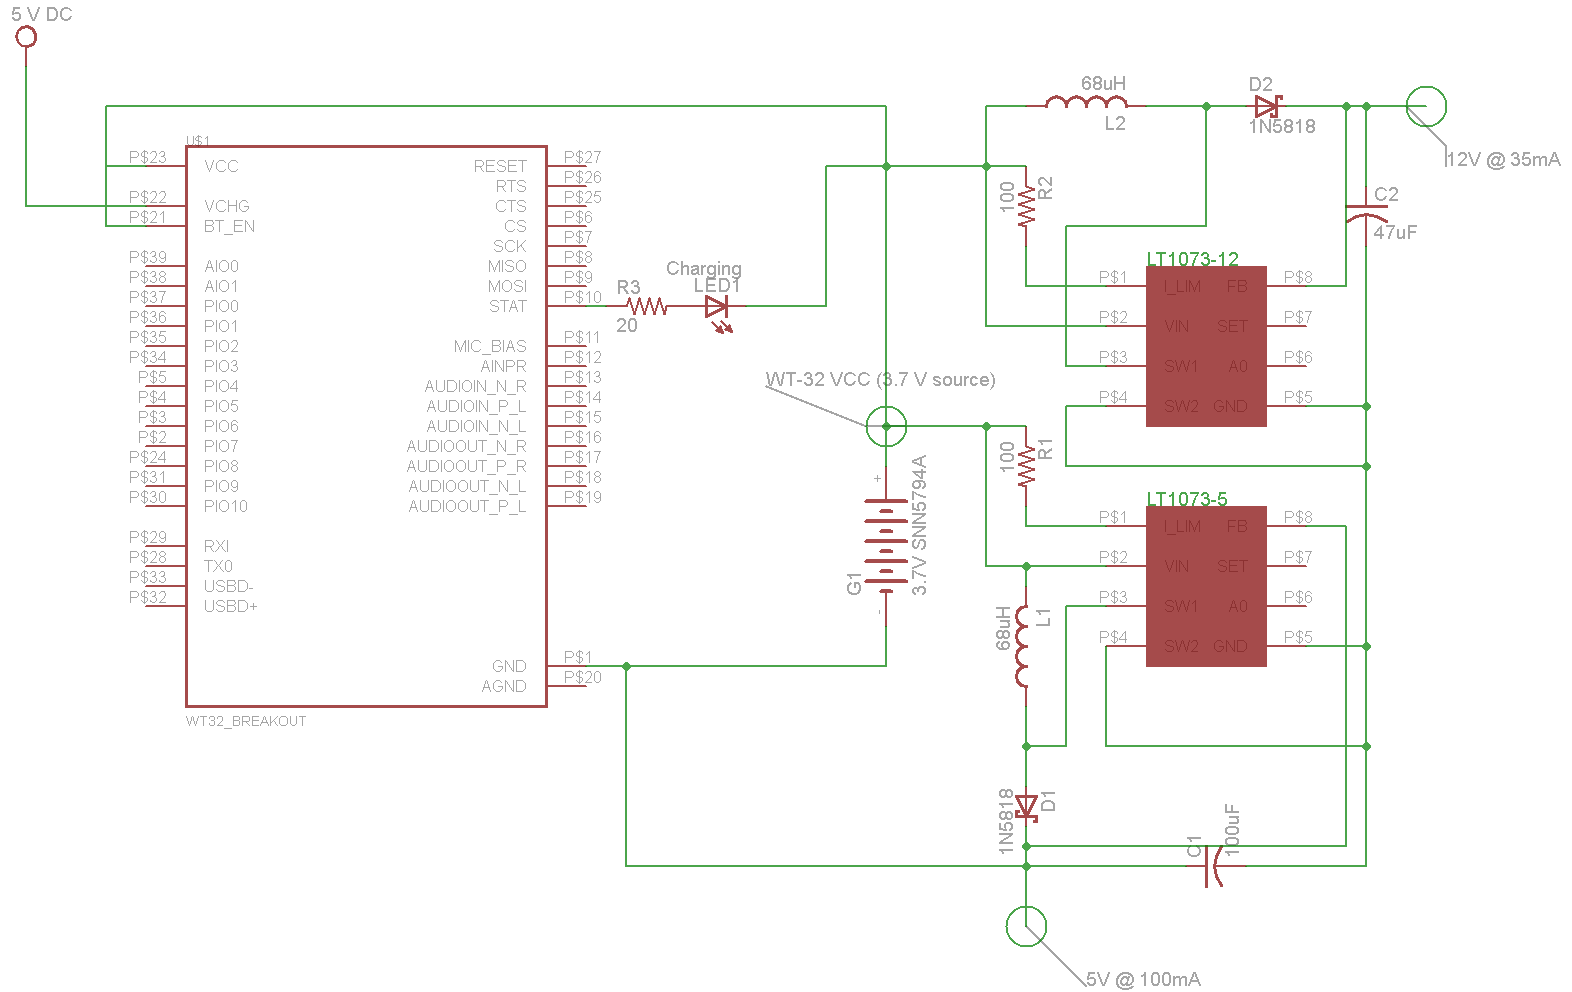
\includegraphics[width=4in]{../drawings/power_final_sch.png}
\caption[Power Supply]{Power supply prototype schematic}
\label{fig:final_power_schematic}
\end{figure}   

It is important to note that while prototyping does not require close quarters for the necessary components, a production model may require a toroidal instead of rod-type inductor in order to reduce the effects of EMI on the analog circuitry. Also, in the interest of cost, simple electrolytic capacitors are used instead of high end Tantalum capacitors. 1N5818 Schottky diodes are suggested for the LT1073 as they have a low forward voltage drop and switch quickly. Extensive trials are still required for this prototype in order to establish actual operating battery life, overall battery life, and possible variation due to noise. The critical power drawing component is the Acquisition Unit which may be characterized by the ATMEGA8515. Refer to Table \ref{tab:battery comparison} to view a best/worst case estimates considering only the two MCU in use. It is notable that it would be very unlikely for both MCUs to be operating constantly. 

\begin{table}[bhp]
\caption[Estimated Operating Time]{Power consumption estimate -  assuming 30\% idle time\cite{ds:ATMEGA8515}}
\small
\begin{center}
\begin{tabular}{l| c c c c}
\setlength{\tabcolsep}{0pt}
	\multirow{2}{*}{Device Operation} & \multirow{2}{*}{Supply ($I_b$)} & Active 
	& Idle & Estimated battery\\
    &                 &	Current($I_b$)   &	Current ($I_d$)                  &life = $(I_b / I_d) x 0.7$\\\hline
	Li-Poly          & 780mAh &													 & &											\\
	One MCU          &        & 12 mA                    & 5.5 mA      & 54.33 hr \\
	Both MCUs        &        & 24 mA                    & 11.0 mA     & 38.01 hr \\    
  Average          &        & 18 mA		                 & 16.5 mA     & 31.11 hr 
\end{tabular}
\end{center}
\label{tab:battery comparison}
\end{table}

\subsection{RoHS Compliance}

Not all components in the power supply prototype are RoHS (Restriction of Hazardous Substances) compliant as many rod-type passives may contain lead. RoHS restricts the use of lead, mercury, cadmium, hexavalent chromium,and polybrominated diphenylether in electronics. Although this standard is not yet enforced in the United States, it may be soon. It is recommended that any production model only use RoHS compliant materials in the interest of a globally accepted product.

\subsection{Power Supply Cost}

The implementation of the power supply requires the purchase of several ultimately unnecessary components for the purposes of testing and to avoid prototyping delays in the event that a component is faulty or damaged. See Table \ref{tab:power_imp_cost_est} for cost estimates to implement the design.

\begin{table}[bhp]
\caption[Implementation Cost]{Power System Implementation%
Cost\cite{web:caddell-burns-price} \cite{web:wt32-price} \cite{web:resistor-price} \cite{web:cap-price}}
\small
\centering
% Table generated by Excel2LaTeX from sheet 'Sheet1'
\begin{tabular}{l|l|l|l|l}
\setlength{\tabcolsep}{1pt}
Product \# & Description & Quantity & Price/Unit & Total \\\hline
\multirow{2}{*}{WRL-08952}  & Bluetooth Breakout & \multirow{2}{*}{1} & \multirow{2}{*}{\$89.95} & \multirow{2}{*}{\$89.95} \\
		   & - Bluegiga WT-32  &          &   &     \\

    1N5818 & Schottky Diode &         20 &     \$0.14 &     \$2.84 \\

    1N4933 & Fast Recovery Power Rectifier &         10 &     \$0.05 &     \$0.53 \\

106CKR050M & Electrolytic Capacitor &         10 &     \$0.05 &     \$0.45 \\

COM-00526  & Voltage Regulator - 3.3V  &          1 &     \$1.95 &     \$1.95 \\

COM-00527  & Voltage Regulator adjustable &          1 &     \$1.95 &     \$1.95 \\

LT1073CN8  & MicroPower DC-DC 		 & \multirow{2}{*}{2} & \multirow{2}{*}{\$3.15} & \multirow{2}{*}{\$6.30} \\
			 &	Converter  &          &      &      \\
LT1073CN8-12  & MicroPower DC-DC 		 & \multirow{2}{*}{2} & \multirow{2}{*}{\$3.15} & \multirow{2}{*}{\$6.30} \\
			 &	Converter (12 VDC FIXED) &          &      &      \\
LT1073CN8-5  & MicroPower DC-DC 		 & \multirow{2}{*}{2} & \multirow{2}{*}{\$3.15} & \multirow{2}{*}{\$6.30} \\
			 & Converter (lead free) &           &   &  \\

   7300-11 & Caddell-Burns 68uH inductor &          2 &     \$5.40 &    \$10.80 \\
   271-308  & 100 pc resistor assortment & 					1 &			\$6.49 &    \$6.49 \\
   276-309  & 5mm red LED								 &					1 &			\$1.49 &    \$1.49 \\
   SNN5794A & Motorola battery pack			 &					1	&			on hand&    onhand \\
Grand Total & & & & \$133.40\\
\end{tabular}   
\label{tab:power_imp_cost_est}
\end{table}

The actual cost for production is much less than prototype implementation as optimal components have been chosen. This cost is further lessened due to the likelihood that large quantities will be ordered, however, the prototype cost estimate shown in Table \ref{tab:power_prod_cost_est} only assumes a minimum number of components required for a single build.

\begin{table}[bhp]
\caption[Production Cost]{Power System Production Cost \cite{web:caddell-burns-price} \cite{web:cap-price} \cite{web:batt-price}}
\small
\centering
% Table generated by Excel2LaTeX from sheet 'Sheet1'
\begin{tabular}{l|l|l|l|l}
\setlength{\tabcolsep}{1pt}
    Part \# & Description &   Quantity &   Per/Unit & Total Cost \\\hline

\multirow{2}{*}{WRL-08952}  & Bluetooth Breakout & \multirow{2}{*}{1} & \multirow{2}{*}{\$89.95} & \multirow{2}{*}{\$89.95} \\
		   & - Bluegiga WT-32  &          &   &     \\
    1N5818 & Schottky Diode &          2 &     \$0.14 &     \$0.28 \\

    G13440 & 100uF dipped Tantalum Capacitor &          1 &     \$1.00 &     \$1.00 \\

     G7102 & 47uF dipped Tantalum Capacitor &          1 &     \$1.00 &     \$1.00 \\

LT1073CN8-12  & MicroPower DC-DC 		 & \multirow{2}{*}{1} & \multirow{2}{*}{\$3.15} & \multirow{2}{*}{\$3.15} \\
			 &	Converter (12 VDC FIXED) &          &      &      \\
LT1073CN8-5  & MicroPower DC-DC 		 & \multirow{2}{*}{1} & \multirow{2}{*}{\$3.15} & \multirow{2}{*}{\$3.15} \\
			 & Converter (lead free) &           &   &  \\

   7300-11 & Caddell-Burns 68uH inductor &          2 &     \$5.40 &    \$10.80 \\

   276-309 & 5mm red LED &          1 &     \$1.49 &     \$1.49 \\

   271-308 & 100 pc resistor assortment &          1 &     \$6.49 &     \$6.49 \\

  SNN5794A & 3.7 V Lithium Ion  & \multirow{2}{*}{1} & \multirow{2}{*}{\$9.95} &\multirow{2}{*}{\$9.95} \\
		   & Rechargeable Battery &    &   & \\
  Grand Total & & & & \$127.26\\

\end{tabular}  
\label{tab:power_prod_cost_est}
\end{table}
